\documentclass[english]{article}
\usepackage[margin=1in]{geometry}
\usepackage{graphicx}
\usepackage{enumerate}
\usepackage{amsmath}
\usepackage{mathabx}
\usepackage{wasysym}
\usepackage{rotating}
\usepackage{float}
\title{Ph 173: Catalog of Papers Read}
\author{Lauren Gilbert}
\begin{document}
\maketitle
\section{Papers Read}
\subsection{Search for a Light Sterile Neutrino at Daya Bay}
\noindent \textbf{The Daya Bay Collaboration} \\
\noindent Phys. Rev. Lett. 113, 141802 (2014) \\

\noindent Placed new limits on $\theta_{41}$, given a 3+1 model with $10^{-3}$ eV$^2 < \Delta m_4^2 < 0.3$ eV$^2$.  Daya Bay detects antineutrinos with inverse beta decay (IBD; $\bar{\nu}_e + p \rightarrow e^- + n$).  They used multiple experiment halls to compare results (e.g. number of IBD events at each hall, energy spectra).  Data was consistent with three neutrino species.  Plots of limits on $\sin\theta_{41}$ and the energy spectrum of inverse beta decay events shown below.

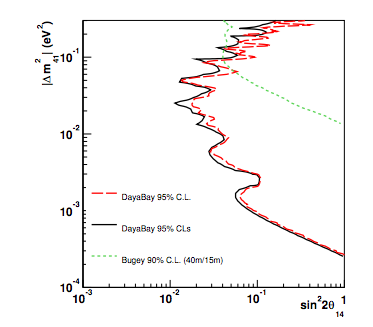
\includegraphics[scale=0.6]{dayabay1.png}
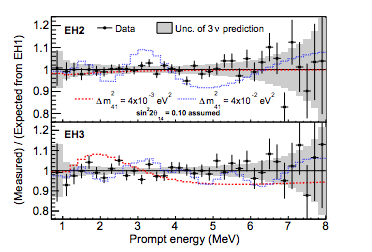
\includegraphics[scale=0.6]{dayabay2.png}

\subsection{Big-Bang Nucleosynthesis in comparison with observed helium and deuterium abundances - possibility of a non-standard model}
\noindent \textbf{R. Ichimasa, R. Nakamura, M. Hashimoto, K. Arai} \\
\noindent Physical Review D, volume 90, eid 023527, 2014 \\

\noindent Standard BBN conditions -- with non-degenerate neutrinos -- are not consistent with new measurements of neutron lifetime and nuclear reaction rates.  They focus on $Y_p$ and $^4$He production, and the mean lifetime of neutrons is taken as 880.1 s, instead of 885.7. \\

\noindent However, scenarios with NACRE II's nuclear measurements and degenerate neutrinos appear to be consistent with Planck's measurements. \\

\noindent References 22-25 may be helpful in implementing chemical potentials for neutrinos in my BBN code. \\

\subsection{Neutrinos, WMAP, and BBN}
\noindent \textbf{Lawrence M. Krauss, Cecilia Lunardini, Christel Smith} \\
\noindent arXiv:1009.4666 [hep-ph]; appears to be an e-print only \\

\noindent This is the most similar paper to my analysis, albeit with WMAP 7 data rather than Planck data.  They focus on the possibility of N$_{eff}\approx$4, which Planck has suggested is not the case, and on neutrino chemical potential.  They do not include flavor mixing, thermalization, and alternate decoupling scenarios.

\noindent I also hadn't realized that a possible future galactic supernovae's neutrino signal could be used to set limits on sterile neutrinos. \\

\subsection{Thermalisation of light sterile neutrinos in the early universe}
\noindent \textbf{Steen Hannestad, Irene Tamborra, Thomas Tram} \\
\noindent JCAP 1207 (2012) 025 \\

\noindent I'm not sure I understand the formal derivation of the quantum kinetic equations -- or, even, that I have the quantum mechanics to understand it.  Similarly, I'm not clear on how one could generate a lepton asymmetry through active-sterile oscillations.  I should also read the references explaining this mechanism.\\

\noindent However, this paper does derive the contribution to N$_{eff}$ from a given lepton asymmetry, which could be useful.  There are very nice limits on $\theta_s$ and $\delta m_s$, if we assume that $\Delta N_{eff} < 1$.  Given the assumptions in Giunti and Laveder (2011; arXiv:1111.1069 [hep-ph]), $\delta N_{eff}$ is entirely consistent with Planck.  However, the Planck results do seem to exclude (or at least strongly disfavor) much of the parameter space for the best-fit model of CMB+LSS with inverted hierarchy. \\

\noindent This paper also has some very interesting plots about the time evolution of both the sterile and active neutrino temperatures.\\

\subsection{Constraints on massive sterile neutrino species from current and future cosmological data}
\noindent \textbf{Elena Giusarma, Martina Corsi, Maria Archidiacono, Roland de Putter, Alessandro Melchiorri, Olga Mena, Stefania Pandolfi} \\
\noindent Phys.Rev.D83:115023, 2011 \\

\noindent While this uses a different BBN code, it contains much the same results that my SURF project did; that is, 3+2 models aren't consistent with BBN when the sterile neutrinos are fully thermalized.  Does not contain much analysis beyond what I did during my SURF. 

\subsection{Additional Light Sterile Neutrinos and Cosmology}
\noindent \textbf{Thomas D. Jacques, Lawrence M. Krauss, Cecilia Lunardini} \\
\noindent Phys. Rev. D 88, 109901 (2013) \\

\noindent Explores possible contributors to $N_{eff}$, particularly fractional contributions.  They focus on partial thermalization of new fermions.  Contains a formal explanation why sterile neutrinos need not be fully thermalized, and that such a 3+2 model can produce $N_{eff} < $4.  Notes that $\Sigma m_\nu$ is also affected by thermalization level; the contribution of each sterile neutrino is $m_\nu\Delta N_{eff}$. \\

\noindent The scenarios in table 1 may be useful to recalculate and compare to Planck data.  This paper assumes that Planck's $N_{eff}$ is the same as $N_{eff}$, which we have determined is not the case; thus, it would be useful to determine if the tension between the theories explored here and Planck's measurements is larger or smaller than reported in this paper. \\

\noindent They also cite a $N_{eff}$ measurement from the South Pole telescope that is inconsistent with the standard model $N_{eff}$; I should look at that measurement and determine if it, like Planck, is calculated by the angle subtended on the sky, and then make appropriate corrections to compare to the theoretical value of $N_{eff}$. \\

\section{To Read}
\subsection{Online}
\begin{itemize}
\item Effects of Long-lived 10 MeV Scale Sterile Neutrino on Primordial Elemental Abundances and Effective Neutrino Number (Ishida, Kusakabe, Okada 2014; arXiv:1403.5995 [astro-ph.CO])
\item Sterile neutrinos with eV masses in cosmology -- how disfavoured exactly? (Hamann, Hannestad, Raffelt, Wong 2011; arXiv:1108.4136 [astro-ph.CO])
\item Implications of 3+1 Short-Baseline Neutrino Oscillations (Giunti and Laveder 2011; arXiv:1111.1069 [hep-ph])
\item Light sterile neutrino production in the early universe with dynamical neutrino asymmetries (Mirizzi, Saviano, Miele, Serpico 2012; arXiv:1206.1046 [hep-ph])
\item Big bang nucleosynthesis limit on N$_\nu$ (Lisi, Sarkar, Villante 1999; arXiv: 9901404 [hep-ph])
\item Constraints on Cosmology from the Cosmic Microwave Background Power Spectrum of the 2500 deg2 SPT-SZ Survey (SPT Collaboration 2014; arXiv:1212.6267 [astro-ph.CO])
\end{itemize}

\subsection{Paper Only}
\begin{itemize}
\item J. Yang, M. S. Turner, D. N. Schramm, G. Steigman, and K. A. Olive, Astrophys. J. 281, 493 11 (1984)
\item N. Terasawa and K. Sato, Astrophys. J. 294, 9 (1985)
\item Cosmological constraints on neutrino degeneracy (H.-S. Kang and G. Steigman; Nucl. Phys. B 372, 494 (1992); technically available online, but is not open-access and Caltech Connect does not have a subscription)
\end{itemize}
\end{document}